
\title{ME314 Final Project}
\author{Jake Ketchum \\
}

\date{\today}
\documentclass[12pt]{article}
\usepackage{amsmath}
\usepackage{graphicx}

\begin{document}
\maketitle

\section{Project Summary}
This project simulates the interactions between a square ball and a 2D stewart platform as shown in figure \ref{frame_diagram}. No external controls have been
applied to the stewart platform. However, it has been made an order of magnitude heavier than the ball to ensure recognizable behavior. For asthetic reasons 'gravity' has been reduced by a factor of 10 and an external wind force was added with which to perturb the system. 

This system is identical to the original proposal with the following exceptions: The proposed control system was omited in the interests of time and the wind force mentioned earlier was included to provide a means of proving the system. None of the proposed extensions of the project were implimented.

In the interests of easier debugging the system was converted to run in near-realtime with an interface for changing the windspeed and system state variable during simulation as shown in figure \ref{gui_default}. The system window depicts an area 400m to a side and runs in real time except during collisions. 



\begin{figure}[h]
\centering
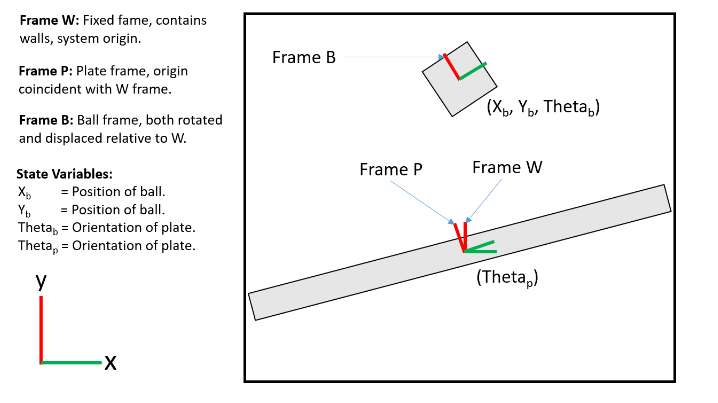
\includegraphics[width=12cm]{diagram.png}
\caption{The system with it's key frames}
\label{frame_diagram}

\end{figure}

\section{Equations of Motion}


\textbf{Euler Lagrange Equations}

\noindent
\textbf{Impact Updates}

The system impacts are defined in a pair of arrays. The first contains CheckLine objects corresponding to each supported collision and  is used for detecting when impacts have occured. The second contains the impact equations themselves and is used in computing the update when an impact has occured.  The impact equation for each condition is defined as the zero vector transformed between a particular point on the ball and a particular point on either the platform or outer frame. By selecting either the x or y coordinate of the transformed vector the appropriate wall can be selected. 

Each CheckLine object is instantiated with it's appropriate transformation, the collision axis, and the allowable collision range along that axis. During instantiation the transformation is lambdified for easy compbutation and the other paramiters are stored. When the check member function is called the lambdified transformation are be used to determine if the ball's point is coincident with the collision axis, and the limits are used to determine if the point falls within the collision line. 

Each time-step, the System iterates throught the entire array of CheckLine objects and calls the check member function for each. If any of the functions return a valid collision the System the then gets the collision equations corresponding to that collision and solves for the update. The update is then applied to the previous time step.  Although the collision checking functions have been lambdified for speed the collision updates are computed symbolically whenever one occurs. 
\begin{figure}[h]
\centering
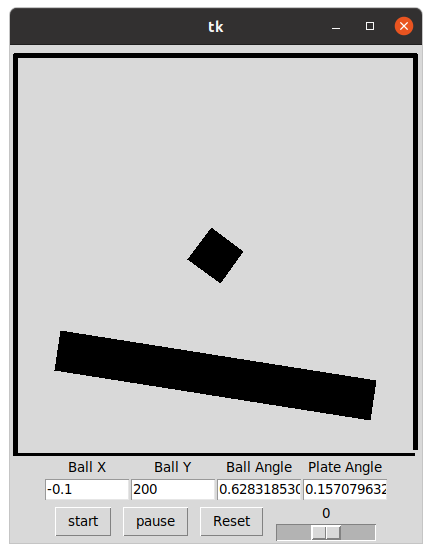
\includegraphics[width=8cm]{gui_no_motion.png}
\caption{The program GUI using the default settings and no wind at startup.}
\label{gui_default}

\end{figure}
\end{document}